\section{Methods}
\label{sec:methods}

This section details the computational methodologies employed to learn and utilize nonlinear deformation modes, addressing the challenges of simulating complex soft tissue behavior. We first review fundamental neural network concepts, which are central to our data-driven learning strategy. Following this, we explore the principles of subspace learning, demonstrating how neural networks can be trained to efficiently represent solutions to constrained physical problems. The core of our proposed method, the 'Neural Modes' architecture, is then introduced, including its specific design and the physics-informed loss functions crucial for its training. Finally, we describe the integration of these learned modes into dynamic simulations and discuss potential directions for extending the framework's capabilities.



\subsection{Neural Network Principles}

A Neural Network (NN) is a mathematical model that achieves statistical generalization drawing inspiration from the human brain. Indeed, it is based on neurons, which are connected one to another, and carry the information from the input to the output \cite{Goodfellow-et-al-2016}.

It is possible to define NN as a function that maps an input to an output, given a set of parameters \( \bm{\theta} \). The function \( \hat{y} = g(\bm{x}; \bm{\theta}) \) is obtained by composing a series of functions \( g_i \) called layers, where each layer is defined as
\begin{equation}
    g_i = \sigma(W_i g_{i-1} + b_i),
\end{equation}
where \( W_i \) is the weight matrix, \( b_i \) is the bias vector and \( \sigma(\cdot) \) is the activation function. The activation function is a non-linear function that allows the network to learn complex patterns in the data.

A neural network is trained using a dataset \( \mathcal{D} = \{(\bm{x}_i, \bm{y}_i)\}_{i=1}^N \), where \( \bm{x}_i \) is the input and \( \bm{y}_i \) is the corresponding target output. The objective is to find the optimal set of parameters \( \bm{\theta} \) that minimizes a loss function \( \mathcal{L} \), which quantifies the discrepancy between the network's predictions and the true outputs. The loss function is defined as:
\begin{equation}
    \mathcal{L}(\bm{\theta}) = \frac{1}{N} \sum_{i=1}^N L(g(\bm{x}_i; \bm{\theta}), \bm{y}_i)
\end{equation}
where \( L \) is a per-sample loss function (e.g., Mean Squared Error). The optimization process aims to find the parameters \( \bm{\theta}^* \) that minimize the overall loss:
\begin{equation}
    \bm{\theta}^* = \argmin_{\bm{\theta}} \mathcal{L}(\bm{\theta}).
\end{equation}
The optimization algorithm used is L-BFGS \cite{Liu_1989}.


To optimize the network parameters, we employ mini-batch gradient descent \cite{hinton2012neural}.  Instead of computing the gradient of the loss function over the entire dataset (batch gradient descent) or for each individual data point (stochastic gradient descent), mini-batch gradient descent strikes a balance by dividing the training data into smaller subsets called mini-batches. For each mini-batch, the loss function \( \mathcal{L}(\bm{\theta}) \) is evaluated, and the gradient \( \nabla_{\bm{\theta}} \mathcal{L}(\bm{\theta}) \) is computed. The parameters \( \bm{\theta} \) are then updated based on this gradient. This approach reduces the computational cost per iteration compared to batch gradient descent and provides a more stable estimate of the gradient compared to stochastic gradient descent, leading to faster convergence.



The gradients required for updating the network parameters are computed using backpropagation. Backpropagation is an algorithm that efficiently computes the gradient of the loss function with respect to each weight in the network. It relies on the chain rule of calculus to propagate the error signal backward through the network, layer by layer.

Specifically, for a layer \( i \) with weights \( W_i \) and bias \( b_i \), the gradients \( \frac{\partial \mathcal{L}}{\partial W_i} \) and \( \frac{\partial \mathcal{L}}{\partial b_i} \) are computed based on the gradient of the loss with respect to the layer's output. These gradients are then used to update the weights and biases of the layer, effectively adjusting the network's parameters to reduce the loss.

The full algorithm is the following one \cite{Rumelhart_Hinton_Williams_1986}
\begin{algorithm}
    \caption{Training of a neural network}
    \begin{algorithmic}
        \State Initialize the parameters \( \bm{\theta} \)
        \While{epoch < max\_epochs}
            \For{mini-batch in dataset}
                \State Perform forward pass computing \( g(\bm{x}; \bm{\theta}) \)
                \State Compute the loss function \( \mathcal{L}(g(\bm{x}; \bm{\theta}), \bm{y}) \)
                \State Perform backward pass computing the gradients of the loss function
                \State Update the parameters using the gradients
            \EndFor
        \EndWhile
    \end{algorithmic}
\end{algorithm}

\subsection{Residual Networks}
Residual Networks (ResNets), introduced by He et al. \cite{He_Zhang_Ren_Sun_2015}, are a neural network architecture designed to overcome the difficulties in training very deep networks. The core idea is the ``skip connection'', also known as a "shortcut connection", which allows the network to bypass one or more layers. This seemingly simple addition has profound implications for the network's ability to learn and generalize.

To understand skip connections, consider a standard neural network where each layer transforms the input it receives from the previous layer. In contrast, a ResNet introduces an identity mapping, where the input of a layer is added to the output of that layer. This is typically implemented using residual blocks.


In a standard neural network, each layer \(f_i\) transforms the output of the previous layer \( \bm{x}_{i-1} \). A residual block, however, learns a residual function \( \mathcal{R}_i(\bm{x}_{i-1}) \). The output of the block \( \bm{x}_i \) is then the sum of the input \( \bm{x}_{i-1} \) (the skip connection) and the learned residual:
\begin{equation}
    \bm{x}_i = \bm{x}_{i-1} + \mathcal{R}_i(\bm{x}_{i-1}).
\end{equation}
The function \( \mathcal{R}_i(\bm{x}_{i-1}) \) typically consists of a few layers (e.g., two fully connected layers with activation functions).

\begin{figure}[H]
    \centering
    \begin{tikzpicture}
        \node[rectangle, draw, minimum width=2cm, minimum height=1cm] (input) at (0,0) {Input $\bm{x}$};
        \node[rectangle, draw, minimum width=2cm, minimum height=1cm, right=of input, node distance=3cm] (layer1) {Layer $\mathcal{R}(\bm{x})$};
        \node[circle, draw, inner sep=2pt, right=of layer1, node distance=2cm] (plus) {$+$};
        \node[rectangle, draw, minimum width=2cm, minimum height=1cm, right=of plus, node distance=2cm] (output) {Output $\bm{x} + \mathcal{R}(\bm{x})$};

        \draw[->] (input) -- (layer1);
        \draw[->] (layer1) -- (plus);
        \draw[->] (plus) -- (output);
        \draw[->] (input) to[out=30,in=150] (plus); % Skip connection
        
        \node[below=0.5cm] at (layer1) {Residual Block};
        
    \end{tikzpicture}
    \caption{A simple illustration of a residual block with a skip connection.}
    \label{fig:residual_block}
\end{figure}

This architecture offers several significant advantages. Primarily, it mitigates the vanishing gradient problem often encountered in deep networks. In very deep standard networks, gradients can become progressively smaller as they are backpropagated through many layers, making it difficult to train the initial layers effectively. Residual connections address this by providing a direct path for the gradient to flow.

Consider the output of a residual block \( \bm{x}_i = \bm{x}_{i-1} + \mathcal{R}_i(\bm{x}_{i-1}) \). When computing the gradient of the loss function with respect to the input of the block \( \bm{x}_{i-1} \), the chain rule gives:
\begin{equation*}
    \frac{\partial \mathcal{L}}{\partial \bm{x}_{i-1}} = \frac{\partial \mathcal{L}}{\partial \bm{x}_i} \frac{\partial \bm{x}_i}{\partial \bm{x}_{i-1}}.
\end{equation*}
The term \( \frac{\partial \bm{x}_i}{\partial \bm{x}_{i-1}} \) is the gradient of the block's output with respect to its input. Due to the skip connection, this gradient is:
\begin{equation*}
    \frac{\partial \bm{x}_i}{\partial \bm{x}_{i-1}} = \frac{\partial}{\partial \bm{x}_{i-1}} (\bm{x}_{i-1} + \mathcal{R}_i(\bm{x}_{i-1})) = I + \frac{\partial \mathcal{R}_i(\bm{x}_{i-1})}{\partial \bm{x}_{i-1}},
\end{equation*}
where \( I \) is the identity matrix. Substituting this back into the loss gradient equation:
\begin{equation*}
    \frac{\partial \mathcal{L}}{\partial \bm{x}_{i-1}} = \frac{\partial \mathcal{L}}{\partial \bm{x}_i} \left( I + \frac{\partial \mathcal{R}_i(\bm{x}_{i-1})}{\partial \bm{x}_{i-1}} \right) = \frac{\partial \mathcal{L}}{\partial \bm{x}_i} + \frac{\partial \mathcal{L}}{\partial \bm{x}_i} \frac{\partial \mathcal{R}_i(\bm{x}_{i-1})}{\partial \bm{x}_{i-1}}.
\end{equation*}
This equation shows that the gradient \( \frac{\partial \mathcal{L}}{\partial \bm{x}_{i-1}} \) is composed of two parts: a direct term \( \frac{\partial \mathcal{L}}{\partial \bm{x}_i} \) that bypasses the residual function \( \mathcal{R}_i \), and a term that goes through \( \mathcal{R}_i \). The presence of the identity term \( I \) in \( \frac{\partial \bm{x}_i}{\partial \bm{x}_{i-1}} \) ensures that the gradient can propagate effectively backward through the network, even if the gradient of the residual part \( \frac{\partial \mathcal{R}_i(\bm{x}_{i-1})}{\partial \bm{x}_{i-1}} \) is small or close to zero. This direct gradient path prevents the overall gradient from vanishing, allowing for the successful training of much deeper networks.
Furthermore, ResNets make it easier for the network to learn identity mappings. If an identity transformation is optimal for a certain part of the network, meaning the layer should ideally just pass its input through, it is simpler for the residual block to achieve this by learning a near-zero residual \( \mathcal{R}_i(\bm{x}_{i-1}) \approx \bm{0} \). This is considerably easier than compelling a stack of non-linear layers to approximate an identity function. Consequently, by addressing the vanishing gradient issue and simplifying the learning of identity or near-identity functions, ResNets enable the successful training of much deeper networks than was previously feasible, often leading to improved performance.

For our Neural Modes framework, ResNets are particularly well-suited and perform a bit better than Fully Connected Networks. We aim to learn non-linear corrections to an existing linear modal basis. The skip connections can be thought of as preserving the input (related to the linear modes), while the residual function learns the necessary nonlinear adjustments. This aligns with our goal of enhancing, rather than completely replacing, the linear modal approximation. The architecture's ability to learn small, incremental changes is beneficial for this physics-informed correction task. 





\subsection{Neural Modes model}
In this work, we employ a deep residual neural network specifically designed to learn non-linear deformation modes. This architecture builds upon traditional fully connected neural networks but incorporates residual connections to facilitate the training of deeper networks and improve performance in capturing nonlinear corrections to linear modal displacements.


\subsubsection{Architecture}
\label{sec:neural_modes_arch}
The Neural Modes architecture is specifically designed to learn non-linear corrections \( \bm{y} \) that enhance a linear modal approximation, which is parameterized by a modal coordinate vector \( \mathbf{z} \). A crucial difference in our implementation, with respect to the original paper \cite{Wang_Du_Coros_Thomaszewski_2024}, is to enforce by design the property that a zero input modal coordinate vector \( \mathbf{z}=\bm{0} \) results in a zero correction output \( \bm{y}=\bm{0} \), i.e., \( \text{model}(\bm{0}) = \bm{0} \). This ensures that in the rest state (corresponding to \( \mathbf{z}=\bm{0} \)), the network does not predict non-linear correction, aligning with physical intuition and simplifying the training process. As discussed in Section \ref{sec:training_neural_modes}, this bias-free architecture led to slightly better results and more stable training compared to using an explicit origin penalty term in the loss function. The specific implementation is a deep residual network, referred to as `ResidualNet', with the following structure:

\begin{itemize}
    \item \textbf{Input:} A modal coordinate vector \( \mathbf{z} \in \mathbb{R}^{\ell_{dim}} \), where \(\ell_{dim}\) is the dimension of the modal input space.
    \item \textbf{Network Core:}
    \begin{itemize}
        \item \textbf{Input Projection Layer:} A linear layer without bias terms that maps the input \( \mathbf{z} \) to a hidden representation of dimension \(d_h\). An activation function (default: Leaky ReLU \cite{xu2015empiricalevaluationrectifiedactivations}) is applied to the output of this projection.
        \item \textbf{Residual Blocks:} A sequence of \(N_{\text{layers}}\) residual blocks. Each block is designed to learn a residual function and consists of:
        \begin{itemize}
            \item Two linear layers, each without bias terms. The input to the block is first passed through a linear layer, followed by an activation function, then a Layer Normalization. This is repeated for the second linear layer and Layer Normalization within the block.
            \item Two Layer Normalization (`LayerNorm`) layers, configured without learnable affine parameters (i.e., no learnable scale or shift).
            \item An activation function (default: Leaky ReLU) applied after each linear transformation within the block, before the Layer Normalization.
            \item A skip connection that adds the input to the residual block to its processed output (after all layers in the block), facilitating gradient flow and learning.
        \end{itemize}
        \item \textbf{Output Projection Layer:} A final linear layer without bias terms that maps the processed hidden representation from the last residual block to the output correction vector \( \bm{y} \). The weights of this layer are initialized to zero.
        \end{itemize}
        \item \textbf{Output:} A nonlinear correction vector \( \bm{y} \in \mathbb{R}^{d_u} \), where \(d_u\) is the dimension of the full displacement space (e.g., number of degrees of freedom in a mesh). This correction \( \bm{y} \) is intended to be added to a linear modal displacement.
        \item \textbf{Zero-Output for Zero-Input Property:} The combined effect of using bias-free linear layers, LayerNorm without learnable affine parameters, and zero-initializing the weights of the output projection layer guarantees that if the input \( \mathbf{z} \) is a zero vector, the network's output \( \bm{y} \) will also be a zero vector. This is crucial for ensuring no artificial correction is applied at the rest state, aligning with physical expectations.
    \end{itemize}



The network learns to map from the reduced modal space (\( \mathbb{R}^{\ell_{dim}} \)) to full-dimensional correction vectors (\( \mathbb{R}^{d_u} \)) that improve the accuracy of the linear modal approximation. This architecture, which we call Neural Modes, can be visualized as a mapping from a low-dimensional modal space to a high-dimensional displacement space, where the neural network learns to correct the linear approximation provided by the modal basis. The following figure \ref{fig:neural_modes_arch} illustrates the architecture:
\begin{figure}[H]    \centering
    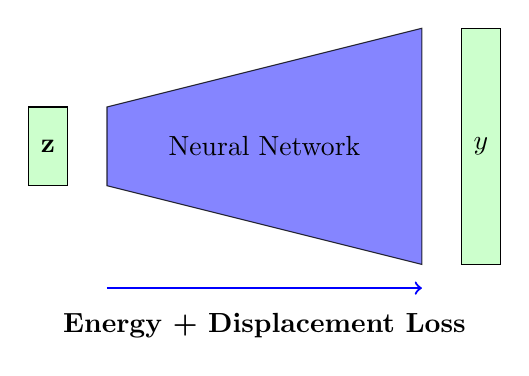
\begin{tikzpicture}
        % Modal coordinate (z)
        \draw[fill=green!20] (-3, 1) rectangle (-2.5,2);
        \node at (-2.75, 1.5) {$\mathbf{z}$}; % Label inside the rectangle
        
        % Displacement (u)
        \draw[fill=green!20] (2.5,0) rectangle (3,3);
        \node at (2.75, 1.5) {$\bm{y}$}; % Label inside the rectangle
        
        % Energy loss transition
        \draw[fill=blue!60,opacity=0.8] (-2,1) -- (2,-0) -- (2,3) -- (-2,2) -- cycle;
        \node at (0,1.5) {Neural Network};
        \node[below] at (0,-0.5) {\textbf{Energy + Displacement Loss}};
        
        % Energy loss arrow
        \draw[thick,blue,->] (-2,-0.3) -- (2,-0.3);
    
    \end{tikzpicture}
    \caption{Neural Modes architecture for learning nonlinear deformation corrections}
    \label{fig:neural_modes_arch}
\end{figure}


\subsection{Subspace Learning}
Here we'll outline the training idea behind the original Neural Modes framework \cite{Wang_Du_Coros_Thomaszewski_2024}, which is based on learning a subspace of equilibrium configurations of the system. This is the approach we used to train in a self-supervised way the Neural Modes network, in order to obtain a comparison with the supervised learning approach we adopted in the previous section.


Let \( \bm{X} \in \mathbb{R}^{n \times d} \) and \( \bm{x} \in \mathbb{R}^{d} \) be the vectors representing the undeformed and deformed configurations of a mesh, respectively. We can characterize equilibrium configurations of the system by constrained energy minimization principles, such as 
\begin{align}
    \label{eq:constrained_energy_minimization}
    \bm{x}^*(\phi, \psi) = \underset{\bm{x}}{\argmin} \quad & E_\phi(\bm{x}) \\
    \text{s.t.} \quad & C_\psi(\bm{x}) = 0, \nonumber
\end{align}
where \( E_\phi \) is the energy function defined by parameters \(\phi\) and \( C_\psi \) is the constraint function with parameters \(\psi\). The solution set \( \bm{x}^*\) constitutes a subspace of the full-dimensional space \( \mathbb{R}^d \). In a classical Finite Element framework, sampling from this subspace is achieved by solving a constrained minimization problem for each configuration. 

Clearly, this approach is computationally expensive, so we need a more efficient way to sample from the subspace.

The idea proposed by \cite{Wang_Du_Coros_Thomaszewski_2024} is to find a Neural Network \( \bm{x}[\theta^*](\phi, \psi) \) that approximates the solution \( \bm{x}^* \), meaning that the problem becomes:
\begin{align*}
    \bm{x}[\theta^*](\phi, \psi) \approx \underset{\theta}{\argmin} \quad & E_\phi(\bm{x}[\theta](\phi, \psi)) \\
    \text{s.t.} \quad & C_\psi(\bm{x}[\theta](\phi, \psi)) = 0.
\end{align*}

Now, defining the nonlinear modes as 
\begin{align}
    \bm{n}(\mathbf{z}) = \bm{l} + \argmin_{\bm{y}} \quad & E_\phi(\bm{X} + \bm{l} + \bm{y}) \\ 
    \text{s.t.} \quad & \bm{l}^T \bm{y} = 0,
\end{align}
where \( \bm{l} \) is the linear mode displacement obtained as
\begin{equation}
    \bm{l} = \sum_{i=1}^m z_i \bm{e}_i,
\end{equation}
where \( \bm{e}_i \) is the $i$-th linear mode and \( z_i \) is the corresponding modal coordinate, we can rewrite the problem \ref{eq:constrained_energy_minimization} as:
\begin{align*}
    \bm{n}[\theta^*](\mathbf{z}) &= \bm{l} + \bm{y}[\theta^*](\mathbf{z}), \\
    \theta^* = \underset{\theta}{\argmin} \quad & E_\phi(\bm{X} + \bm{l} + \bm{y}[\theta](\mathbf{z})) \\
    \text{s.t.} \quad & \bm{l}^T \bm{y}[\theta](\mathbf{z}) = 0.
\end{align*}

Now we define a suitable function that will serve as a loss function for the self-supervised training of the neural network. The loss function is defined as:
\begin{equation}
    \mathcal{L}(\theta) = \mathbb{E}_{\mathbf{z}} \left[ E(\bm{X} + \bm{l}(\mathbf{z}) + \bm{y}[\theta](\mathbf{z})) + \alpha_1 \bm{l}(\mathbf{z})^T \bm{y}[\theta](\mathbf{z}) + \alpha_2 \sum_{j \in \mathcal{B}} \|(\bm{X} + \bm{l}(\mathbf{z}) + \bm{y}[\theta](\mathbf{z}))_j\|^2 \right],
\end{equation}
where \( E \) is the internal energy of the deformed configuration, \( \bm{l}(\mathbf{z}) \) is the linear mode displacement for modal coordinates \( \mathbf{z} \), \( \bm{y}[\theta](\mathbf{z}) \) is the nonlinear correction predicted by the network with parameters \( \theta \), \( \mathcal{B} \) is the set of boundary nodes with fixed displacement, and \( \alpha_1 \) and \( \alpha_2 \) are hyperparameters. The first term minimizes the internal strain energy, the second term enforces orthogonality between the linear mode displacement and the nonlinear correction, and the third term penalizes deviations from the required boundary conditions at the fixed nodes.




\subsection{Neural Modes Training} % fix this
\label{sec:training_neural_modes}
The paper we took inspiration from, by Wang et al. \cite{Wang_Du_Coros_Thomaszewski_2024}, uses a data-free approach to learn the nonlinear modes, which is based on the idea of minimizing the internal energy of the deformed configuration. To do so, they provide two strategies for sampling the latent space, which is the space of the modal coordinates \( \mathbf{z} \). The first strategy is to sample the latent space uniformly, with each component of the modal coordinate vector \( \mathbf{z} \) being sampled uniformly from the same range. The second strategy is a stochastic sampling approach, where, at each epoch, a new random vector is generated, and the network is trained to minimize the energy loss for that specific configuration. Also in this case, the range of values is the same for each component of the modal coordinate vector \( \mathbf{z} \).

A key observation in the original work was that the network had a tendency to learn a non-zero correction even when the input modal coordinate vector was zero (\(\mathbf{z} = \bm{0}\)), which corresponds to the rest position. To address this, Wang et al. \cite{Wang_Du_Coros_Thomaszewski_2024} incorporated an explicit origin penalty term into their loss function to encourage the network output to be zero at the origin.

Our numerical results show that the data-free approach performs well, as long as the range from which the modal coordinate vector \( \mathbf{z} \) was sampled was not too large, similarly to how linear modes work. In subsection \ref{sec:sampling_modal_space}, we will discuss more in detail why sampling the latent space uniformly can lead to unrealistic deformations. Since finding a good sampling strategy is crucial for the success of the Neural Modes framework and the deformation range we were aiming to cover was quite large, leading to very difficult energy landscapes for the optimizer, we decided to adopt a different training strategy that keeps some ideas from the original paper but loses the data-free approach in favor of a supervised learning strategy.

Instead of using an explicit origin penalty in the loss function as in \cite{Wang_Du_Coros_Thomaszewski_2024}, we achieved the desired property that a zero input modal coordinate vector \( \mathbf{z}=\bm{0} \) results in a zero correction output \( \bm{y}=\bm{0} \) by design through a bias-free network architecture. As discussed in Section \ref{sec:neural_modes_arch}, this architectural choice centers the network's output at the origin. Through our experimentation, we observed slightly better results and more stable training by adopting this bias-free architecture compared to using an explicit origin penalty term in the loss function.

The dataset for our supervised training approach is generated starting from FEM simulations of the object of interest, applying the forces described in the Modal Forces section \ref{sec:modal_forces}. The dataset is built by linking the modal coordinate vector \( \mathbf{z} \) to the corresponding full nonlinear deformation \( \bm{u} \) of the object along with its internal energy \( E(\bm{u}) \). The dataset is structured as pairs of input-output samples, which are then fed to the neural network by randomly picking a batch of samples for each training epoch.

The internal energy \( E(\bm{u}) \) of the deformed configuration is computed following this equation:


\begin{equation}
    E(\bm{u}) = \int_{\Omega} \Psi(\bm{F}(\bm{u})) \, d\Omega,
\end{equation}
where $\Psi$ is the Neo-Hookean strain energy density function (as defined in Equation \eqref{eq:neo_hookean_energy}). In the context of the loss function, $\bm{u}$ refers to the predicted total displacement $\bm{X} + \bm{l} + \bm{y}$.



The training process for the Neural Modes Network is based on minimizing a combination of loss functions that tries to capture the essential physical properties of the deformation modes. The loss function is built around three main components:
\begin{enumerate}
    \item \textbf{Energy Loss}: To train the neural network to accurately predict the internal energy of deformed configurations, we employ a Mean Squared Error (MSE) loss function.  However, instead of directly comparing the predicted energy with the actual energy, we compute the MSE between the base-10 logarithms of these values. This transformation serves two primary purposes: First, the logarithmic transformation compresses the range of energy values, which can span several orders of magnitude, providing scale invariance. By using $\log_{10}(E)$, we reduce the sensitivity of the loss function to large absolute differences in energy, particularly at higher energy levels. This ensures that the network learns effectively across different energy scales, preventing the dominance of high-energy configurations in the training process. Second, the logarithm function helps to create a smoother loss landscape. The original energy values might lead to a highly irregular loss surface, making it difficult for gradient-based optimization algorithms to converge. By using the logarithm, we transform the error surface into a more smooth shape, facilitating more stable and efficient training, since the logarithm reduces the impact of outliers and sharp changes in the energy values, leading to more consistent gradients during optimization.

    The energy loss is thus defined as:
    \begin{equation}
        \mathcal{L}_{E} = \frac{1}{N} \sum_{i=1}^N (\log_{10}(E(\bm{X} + \bm{l} + \bm{y})) - \log_{10}(E_{FEM}))^2,
    \end{equation}
    where \( E \) is the internal energy of the deformed configuration \( \bm{X} + \bm{l} + \bm{y} \), computed using the finite element method, \( E_{\text{pred}} \) is the predicted energy by the network, \( \bm{X} \) is the undeformed configuration, and \( \bm{l} \) is the linear mode displacement.  The vector \(\bm{y}\) represents the nonlinear displacement field predicted by the neural network.
    
    \item \textbf{Displacement Loss}: the MSE loss between the predicted displacement \( \bm{X} + \bm{l} + \bm{y} \) and the ground truth displacement \( \bm{u} \):
    \begin{equation}
        \mathcal{L}_u = \frac{1}{N} \sum_{i=1}^N \|\bm{X} + \bm{l} + \bm{y} - \bm{u}\|^2,
    \end{equation}
    where \( \bm{u} \) is the ground truth displacement obtained from the FEM simulation.
    \item \textbf{Orthogonality Loss}: ensures that the nonlinear correction \( \bm{y} \) is orthogonal to the linear mode displacement \( \bm{l} \):
    \begin{equation}
        \mathcal{L}_{ortho} = \frac{1}{N} \sum_{i=1}^N (\bm{l}^T \bm{y})^2,
    \end{equation}

        \item \textbf{Boundary Condition Penalty}: enforces the displacement boundary conditions on the deformed configuration. For nodes \( j \) belonging to the set of boundary nodes \( \mathcal{B} \), where the displacement is fixed (e.g., to zero), this loss penalizes deviations from the required displacement. It is defined as the sum of squared displacements at the boundary nodes:
        \begin{equation}
            \mathcal{L}_{BC} = \frac{1}{N} \sum_{i=1}^N \sum_{j \in \mathcal{B}} \|(\bm{X}_i + \bm{l}_i + \bm{y}_i)_j\|^2,
        \end{equation}
        where \( (\bm{X}_i + \bm{l}_i + \bm{y}_i)_j \) is the predicted displacement vector at node \( j \) for the \( i \)-th sample in the batch. This term encourages the network to predict corrections \( \bm{y} \) such that the total displacement \( \bm{X} + \bm{l} + \bm{y} \) satisfies the fixed boundary conditions.
    
\end{enumerate}

The total loss function is a weighted sum of these individual losses:
\begin{equation}
    \mathcal{L} = \alpha_1 \mathcal{L}_E + \alpha_2 \mathcal{L}_u + \gamma_1 \mathcal{L}_{ortho} + \gamma_2 \mathcal{L}_{BC},
\end{equation}
where $\gamma_1$ and $\gamma_2$ are weight parameters that balance the importance of the orthogonality and boundary condition penalty terms, respectively, and $\alpha_1$ and $\alpha_2$ are hyperparameters that control the relative importance of the energy and displacement losses. 





\subsection{Sampling the Modal Space}
\label{sec:sampling_modal_space}
One of the main challenges for this method is finding a good way to sample the \(z\) vector that will be used as input for the neural network. Here are two examples that shows how choosing randomly the \(z\) vector can lead to unrealistic results. 
\begin{figure}[H]
    \centering
    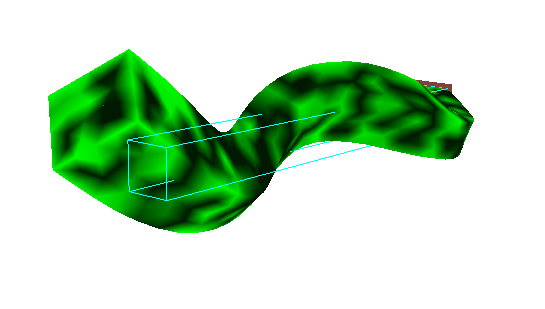
\includegraphics[width=0.4\textwidth]{Images/z_random.png}
    \caption{Example of a bad sampling of the modal space, the reference shape is the light blue outline. The beam is unnaturally twisted and at the same time double bent, which is not a physically plausible deformation.}
    \label{fig:bad_sampling}
\end{figure}

In this example, the random \(z\) vector has large values in its latter components. These components represent higher-frequency deformation modes, which naturally contain more strain energy. Using these modes with high amplitudes often creates physically unrealistic or extreme configurations. This shows why random sampling across all components of \(z\) can lead to unrealistic deformations.

A better sampling approach considers the physical meaning of each mode. The first components of \(z\) typically correspond to lower-frequency, global deformation modes $\varphi$ that represent major shape changes with less energy. Later components represent higher-frequency, localized, and more energetic modes. 

For more effective sampling of the modal space, we can implement a strategic approach to generating the \(z\) vectors. This approach involves assigning larger coefficient values to the first components of the vector, which typically correspond to the fundamental, lower-frequency deformation modes, while progressively reducing the magnitude of values assigned to later components. By structuring our sampling in this manner, the resulting deformations tend to be significantly more physically realistic and energetically feasible in real-world scenarios. This methodical sampling focuses the neural network's training process on common, naturally occurring deformation patterns rather than directing computational resources toward unlikely, high-energy configurations that rarely manifest in practical applications.


We decided to use a supervised learning approach, where the dataset is generated from FEM simulations of the object of interest, meaning that the modal coordinate vector \( \mathbf{z} \) that the network receives as input is necessarily a valid modal coordinate vector, in the sense that describes a physically plausible deformation of the object. The dataset is built by linking the modal coordinate vector \( \mathbf{z} \) to the corresponding full nonlinear deformation \( \bm{u} \) of the object along with its internal energy \( E(\bm{u}) \). 

\subsection{Dynamic Simulation with Neural Modes}
\label{sec:subspace_dynamics}
One of the strengths of this framework is the possibility to employ it for dynamic simulations at a fraction of the cost of a full order simulation. Once we have trained the network to map the modal coordinates vector to a full displacement, we can take advantage of this.
For dynamic simulations, the Neural Modes framework solves an optimization problem at each time step. Given the current and previous displacement states $\bm{u}_n$ and $\bm{u}_{n-1}$, the modal coordinates for the next time step $\mathbf{z}_{n+1}$ are computed by minimizing the total energy of the system, including inertial terms:
\begin{equation}
    \mathbf{z}_{n+1} = \underset{\mathbf{z}}{\argmin} \frac{1}{2h^2} \|\bm{n}(\mathbf{z}) - 2\bm{u}_n + \bm{u}_{n-1}\|_{\bm{M}}^2 + \mathcal{E}(\bm{n}(\mathbf{z})),
    \label{eq:optimization_problem}
\end{equation}
where $\bm{n}(\mathbf{z})$ represents the complete displacement field (undeformed configuration $\bm{X}$ plus linear modes $\bm{l}(\mathbf{z})$ plus nonlinear correction $\bm{y}(\mathbf{z})$), $h$ is the time step, $\bm{M}$ is the mass matrix, and $\mathcal{E}(\cdot)$ is the total potential energy of the configuration. The total potential energy $\mathcal{E}(\bm{u})$ is defined as the internal strain energy $E(\bm{u})$ minus the work done by external forces $\bm{f}^{ext}$:
\[\mathcal{E}(\bm{u}) = E(\bm{u}) - (\bm{f}^{ext})^T \bm{u}.\]
 This optimization problem is typically solved using the L-BFGS-B algorithm \cite{Liu_1989}.






\subsection{Force generation with Modal Forces}
\label{sec:modal_forces}

To validate the Neural Modes framework and generate physically meaningful training data, we employ a modal force generation approach that leverages the principal deformation modes of the mechanical system. This method addresses the challenge of creating external forces that produce representative deformations while maintaining the nonlinear capabilities essential for large deformation scenarios \cite{odotDeepPhysicsPhysicsAware2021}.

\subsubsection{Mathematical Derivation and Linearization Process}
The foundation of our modal force approach lies in the linearization of the nonlinear finite element equilibrium equations. Starting from the weak form of the hyperelastic boundary value problem, we seek displacement $\bm{u}$ such that:
\begin{equation}
    \int_{\Omega} \bm{P}(\bm{u}) : \nabla \bm{w} \, d\Omega = \int_{\Omega} \bm{f} \cdot \bm{w} \, d\Omega + \int_{\Gamma_N} \bm{h} \cdot \bm{w} \, d\Gamma \quad \forall \bm{w} \in V,
    \label{eq:weak_form_modal}
\end{equation}
where $\bm{P}(\bm{u})$ is the first Piola-Kirchhoff stress tensor, $\bm{f}$ represents body forces, and $\bm{h}$ are traction forces on the Neumann boundary $\Gamma_N$.

In the finite element discretization, this leads to the nonlinear system:
\begin{equation}
    \bm{R}(\bm{u}) = \bm{f}^{int}(\bm{u}) - \bm{f}^{ext} = \bm{0},
    \label{eq:nonlinear_system}
\end{equation}
where $\bm{f}^{int}(\bm{u})$ are the internal forces (functions of displacement) and $\bm{f}^{ext}$ are the external forces. The residual vector $\bm{R}(\bm{u})$ represents the out-of-balance forces.

To solve this nonlinear system \eqref{eq:nonlinear_system}, we employ the Newton-Raphson method \cite{Dedieu_2015}, which requires linearization around the current configuration $\bm{u}^k$:
\begin{equation}
    \bm{R}(\bm{u}^k + \Delta\bm{u}^k) \approx \bm{R}(\bm{u}^k) + \frac{\partial \bm{R}}{\partial \bm{u}}\bigg|_{\bm{u}^k} \Delta\bm{u}^k = \bm{0}.
    \label{eq:newton_raphson}
\end{equation}

The tangent stiffness matrix is defined as:
\begin{equation}
    \mathbb{K}(\bm{u}^k) = \frac{\partial \bm{R}}{\partial \bm{u}}\bigg|_{\bm{u}^k} = \frac{\partial \bm{f}^{int}}{\partial \bm{u}}\bigg|_{\bm{u}^k},
    \label{eq:tangent_stiffness}
\end{equation}
leading to the linearized system at each Newton iteration:
\begin{equation}
    \mathbb{K}(\bm{u}^k) \Delta\bm{u}^k = -\bm{R}(\bm{u}^k) = \bm{f}^{ext} - \bm{f}^{int}(\bm{u}^k).
    \label{eq:linearized_system}
\end{equation}

For our modal force generation, we consider the linearization at the rest configuration $\bm{u}^0 = \bm{0}$, where the internal forces vanish: $\bm{f}^{int}(\bm{0}) = \bm{0}$. This simplifies the linearized system \eqref{eq:linearized_system} to:
\begin{equation}
    \mathbb{K}(\bm{0}) \Delta\bm{u}^0 = \bm{f}^{ext}.
    \label{eq:linearized_system_rest}
\end{equation}

\subsubsection{Modal Decomposition and Force Generation}

The tangent stiffness matrix at the rest configuration $\mathbb{K} = \mathbb{K}(\bm{0})$ can be decomposed using eigenvalue analysis:
\begin{equation}
    \mathbb{K} = \boldsymbol{\Phi} \boldsymbol{\Lambda} \boldsymbol{\Phi}^T,
    \label{eq:eigen_decomposition}
\end{equation}
where $\boldsymbol{\Phi} = [\bm{\phi}_1, \bm{\phi}_2, \ldots, \bm{\phi}_n]$ contains the eigenvectors (deformation modes) and $\boldsymbol{\Lambda} = \text{diag}(\lambda_1, \lambda_2, \ldots, \lambda_n)$ contains the corresponding eigenvalues.

From the linearized equilibrium equation \eqref{eq:linearized_system_rest}, we can express:
\begin{align}
    \mathbb{K} \Delta\bm{u}^0 &= \bm{f}^{ext} \nonumber \\
    \boldsymbol{\Phi} \boldsymbol{\Lambda} \boldsymbol{\Phi}^T \Delta\bm{u}^0 &= \bm{f}^{ext} \nonumber \\
    \boldsymbol{\Phi} (\boldsymbol{\Lambda} \boldsymbol{\Phi}^T \Delta\bm{u}^0) &= \bm{f}^{ext}.
    \label{eq:modal_force_derivation}
\end{align}

Defining the modal coefficients as $\bm{q} = \boldsymbol{\Lambda} \boldsymbol{\Phi}^T \Delta\bm{u}^0$, we obtain the fundamental relationship:
\begin{equation}
    \bm{f}^{ext} = \boldsymbol{\Phi} \bm{q}.
    \label{eq:modal_force_form}
\end{equation}

This fundamental relationship allows us to generate external forces by selecting appropriate modal coefficients $\bm{q}$. Each component $q_i$ represents the amplitude of the $i$-th deformation mode in the applied force pattern. We then apply these external forces to our problem \ref{eq:static_problem} and solve it using a FEM solver to generate our dataset.



The modal force generation methodology offers several significant advantages that directly support the development and validation of our Neural Modes framework. First, the approach ensures physical meaningfulness in the generated test cases. Since the forces are derived from the principal deformation patterns of the mechanical system (as shown in \eqref{eq:modal_force_form}), the resulting displacements naturally exhibit the characteristic behavior of the material under consideration. This is particularly important for soft tissue simulation, where unrealistic deformation patterns can compromise the validity of the learned model.

The method also provides controlled deformation generation capabilities. By systematically selecting specific combinations of modal coefficients $\bm{q}$ in \eqref{eq:modal_force_form}, we can generate comprehensive datasets that span the most significant deformation modes of the system. This systematic approach allows us to ensure adequate coverage of the deformation space while avoiding the computational expense of exhaustive sampling. The ability to control the relative contributions of different modes enables us to focus the training process on the most relevant aspects of the mechanical behavior.

Furthermore, the modal force approach preserves material properties throughout the generation process. Since the modal basis $\boldsymbol{\Phi}$ is directly derived from the material's stiffness matrix $\mathbb{K}$ (via the eigenvalue decomposition in \eqref{eq:eigen_decomposition}), which incorporates the constitutive relationships and geometric configuration, the generated forces inherently respect these fundamental characteristics without requiring manual calibration or parameter tuning. This automatic consistency reduces the likelihood of introducing artifacts or bias in the training data.

Despite utilizing linear modal analysis for force generation (as seen in \eqref{eq:modal_force_form}), the framework retains full nonlinear capability in the solution process. The modal decomposition serves only to structure the external loading; the actual deformation computation employs the complete nonlinear finite element formulation \eqref{eq:nonlinear_system}, preserving all geometric and material nonlinearities. This approach allows us to leverage the computational efficiency of modal analysis while maintaining the accuracy required for large deformation scenarios.

Finally, modal forces provide an ideal validation framework for the Neural Modes network. Since we possess analytical knowledge of the modal responses and can systematically vary the input conditions using $\bm{q}$ in \eqref{eq:modal_force_form}, we can rigorously assess the network's ability to capture both the linear modal behavior and the nonlinear corrections. This controlled environment enables us to verify that the learned corrections indeed improve upon the linear modal approximations and to identify potential limitations or areas for improvement in the network architecture or training process. The validation process is done by computing the Root Mean Square Error (RMSE) between the predicted displacements from the Neural Modes network and the full nonlinear deformations. The RMSE is defined as:
\begin{equation}
    RMSE = \sqrt{\frac{1}{N}\sum_{i=1}^N (\bm{u}_i^{full} - \bm{u}_i^{reduced})^2},
    \label{eq:rmse}
\end{equation}
where $N$ is the number of nodes in the mesh, $\bm{u}_i^{full}$ is the displacement field computed with the full model and $\bm{u}_i^{reduced}$ is the displacement field computed with the reduced model.

For validation purposes, we generate test cases by following two different directions. We perform validation testing either by applying a completely random force vector or we generate a random sample of the modal coefficient vector $\bm{q}$ and, in both cases, compute the corresponding full nonlinear deformation using finite element analysis.
Testing with modal forces ensures that, even in the case of highly irregular geometries, we are evaluating the performance of the Neural Modes framework against what is most similar to the real world data, as sometimes random forces generate completely unrealistic scenarios.

This approach also facilitates the generation of training data that focuses on the most energetically favorable deformation patterns, complementing the strategic sampling of modal coordinates discussed earlier. By ensuring consistency between the force generation and the modal coordinate sampling, we create a coherent framework for both training and validation of the Neural Modes network.

